\chapter[Guia de Uso]{Guia de Uso}

Nesse capítulo é apresentado como utilizar o SVN, através da explicação das primeiras configurações e das principais funcionalidades.

\section{Passo a passo para o primeiro contato com a ferramenta}

Nessa seção são apresentadas as configurações e os passos iniciais para a criação de um repositório utilizando o SVN. Nessa seção serão tratados:

\begin{itemize}

\item Criação de um repositório:

  \subitem Estrutura inicial do repositório;
  \subitem Estrutura recomendada do repositório;
  \subitem Configuração de acesso a um repositório;

\item Disponibilização de um repositório;

\item Acesso a um repositório;

\item Cópias de trabalho;
    \subitem Operações principais;

\end{itemize}

\subsection{Criando um repositório}

Agora que o SVN já está instalado, de acordo com \citeonline{svn-book}, para criação de um repositório deve ser dado o seguinte comando:

\begin{centering}

\colorbox{Gray}{
\begin{minipage}{250px}
  \textbf{svnadmin create <nome do repositorio>}

\end{minipage}
}
\end{centering}

Para importar uma pasta para o repositório, de acordo com \citeonline{wiki-svn}, deve ser dado o seguinte comando:


\begin{centering}

\colorbox{Gray}{
\begin{minipage}{450px}
  \textbf{svn import /caminho/da/pasta/a/ser/copiada file:///caminho/do/repositorio}

\end{minipage}
}
\end{centering}

\subsubsection{O repositório}

De acordo com \citeonline{svn-book}, quando você cria um repositório no SVN ele contém a estrutura de pastas da Figura \ref{fig:estrutura}.

\begin{figure}[!htb]
\centering
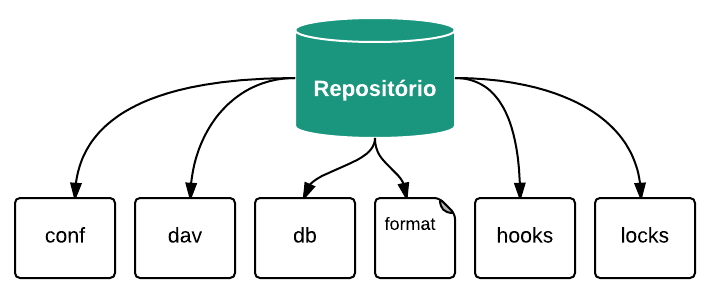
\includegraphics[scale=1]{figuras/repositorio.png}
\caption{Estrutura do repositório. Baseado em \cite{svn-book}}
\label{fig:estrutura}
\end{figure}

\pagebreak
\label{estrutura}
\begin{itemize}

\item conf: Pasta que contém arquivos de configuração do repositório.

\item dav: Pasta que contém arquivos utilizados pelo mod\_dav\_svn.

\item db: Pasta que armazena os dados versionados.

\item format: Arquivo que indica o número da versão do repositório.

\item hooks: Pasta que contém modelos de scripts

\item locks: Pasta para arquivos bloqueados, é utilizado no rastreamento dos acessos ao repositório.

\end{itemize}


O repositório pode ser configurado com a estrutura de pastas que o usuário desejar, todavia existe um padrão recomendado que pode ser visto na Figura
\ref{fig:estrutura_repo}.

\begin{figure}[!htb]
\centering
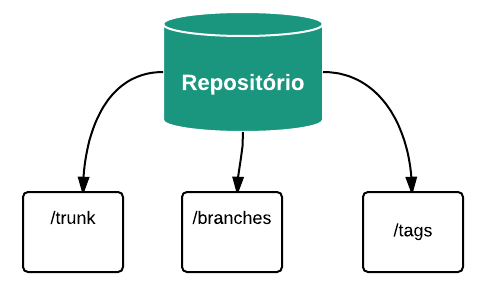
\includegraphics[scale=1]{figuras/estrutura_repo.png}
\caption{Estrutura recomendada do repositório. Baseado em \cite{svn-book}}
\label{fig:estrutura_repo}
\end{figure}

\begin{itemize}
  \item trunk: Pasta principal que contém os arquivos do repositório, é onde fica o projeto testado e sem erros. \cite{wiki-svn}

  \item branches: Pasta utilizada para guardar os arquivos do repositório, "onde você poderá usar para trabalhar em uma nova feature e depois fazer um merge dela com o mainline trunk". \cite{wiki-svn};

  \item tags: Pasta que armazena "snapshots da data do Release de uma dada versão". \cite{wiki-svn}
\end{itemize}

Para criar essa estrutura deve ser dado o comando a seguir para cada uma das pastas: \cite{wiki-svn}

\begin{centering}

\colorbox{Gray}{
\begin{minipage}{280px}
  \textbf{svn mkdir file:///caminho/do/repositorio/pasta}
\end{minipage}
}

\end{centering}

\subsubsection{Configurando o acesso ao repositório}
\label{secao_acesso}
Para configurar o controle de acesso ao repositório devem ser editados os arquivos: \cite{wiki-svn}

\begin{centering}
\colorbox{Gray}{
\begin{minipage}{250px}
  \textbf{caminho/do/repositorio/conf/svnserve.conf}
  \textbf{caminho/do/repositorio/conf/passwd}
\end{minipage}
}
\end{centering}

No arquivo \textit{svnserve.conf} deve ser descomentada a linha \textbf{password-db = passwd} e no arquivo \textit{svnserve.conf}
deve ser escrito o nome do usuário e a senha da seguinte forma: \textbf{usuário = senha}. \cite{wiki-svn}

\begin{centering}
Exemplo:

\colorbox{Gray}{
\begin{minipage}{100px}

  \textbf{usuario1 = 12345}
\end{minipage}
}
\end{centering}

\subsection{Disponibilizando um repositório}

Um repositório pode ser mantido apenas localmente e seu acesso torna-se restrito à máquina a qual ele foi criado. Mas isso não é muito vantajoso, dessa forma um repositório deve ser disponibilizado em um servidor para que as pessoas possam acessá-lo de qualquer lugar. As opções de servidor podem ser vistas no anexo \ref{servidores}.

\subsection{Acessando um repositório}

  Os repositórios criados para controle de versão com o SVN são acessados através de URLs, seguindo os seguintes padrões: \cite{svn-book}

\begin{centering}

\textbf{Para o servidor:} É especificado o nome do servidor e a porta.

\colorbox{Gray}{
\begin{minipage}{220px}
  \textbf{http://svn.example.com:9834/repos}
\end{minipage}
}

\textbf{Para repositórios locais:} a URL ganha o prefixo \textit{file:}. Podem ser escritos com o nome do servidor, ou sem. E de acordo com \citeonline{wiki-svn}, para acessar repositórios locais deve apenas digitar o comando \textbf{svn co url\_definida}.
\end{centering}

\begin{multicols}{2}


\flushright{O nome do servidor como \textit{localhost}:

\colorbox{Gray}{
\begin{minipage}{210px}
  \textbf{file://localhost/caminho/repositorio}
\end{minipage}
}
}

Ou sem especificação do servidor:

\colorbox{Gray}{
\begin{minipage}{200px}
\flushleft{
  \textbf{file:///caminho/repositorio}
}
\end{minipage}
}

\end{multicols}

As possíveis URLs de acesso podem ser vistas na Tabela \ref{tab:urls}.

\begin{table}[!h]
\centering
\caption{URLs de acesso ao repositório. Fonte: \cite{svn-book}}
\label{tab:urls}
\begin{tabular}{|l|l|}
\hline
\rowcolor[HTML]{01796F}
{\color[HTML]{000000} \textbf{Esquema}} & {\color[HTML]{000000} \textbf{Método de Acesso}}                             \\ \hline
file:///                                & acesso direto ao repositório (em um disco local).                            \\ \hline
http://                                 & acesso via protocolo WebDAV em um servidor Apache especialmente configurado. \\ \hline
https://                                & mesmo que http://, mas com encriptação SSL.                                  \\ \hline
svn://                                  & acesso via protocolo próprio em um servidor svnserve.                        \\ \hline
svn+ssh://                              & mesmo que svn://, mas através de um túnel SSH.                               \\ \hline
\end{tabular}
\end{table}



\subsection{Cópias de trabalho}

O SVN trabalha com cópias de trabalho. Uma cópia de trabalho consiste na mesma estrutura do repositório para uso privado. Ou seja, é a cópia local do repositório que pode ser editada pelo usuário.

Para criar uma cópia de trabalho deve ser digitado o seguinte comando: \citeonline{svn-book}


\begin{centering}
\colorbox{Gray}{
\begin{minipage}{320px}
  \textbf{svn checkout http://svn.example.com:9834/repositorio}
\end{minipage}
}

\end{centering}

\subsubsection{Como funciona a relação entre o repositório e a cópia de trabalho?}

\begin{figure}[!htb]
\centering
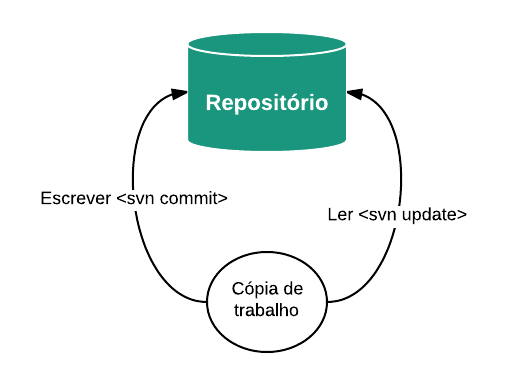
\includegraphics[scale=1]{figuras/repositorio_copia.png}
\caption{Comunicação entre cópia de trabalho e repositório. Baseado em \cite{svn-book}}
\end{figure}


Para que os outros membros do projeto tenham acesso ao que foi produzido na cópia de trabalho, o SVN permite que o usuário escreva no repositório as alterações feitas
e para ter acesso às atualizações feitas por outros membros, é permitido ao usuário ler o repositório. \cite{svn-book}

\begin{multicols}{2}


\flushright{Para escrever}:{

\colorbox{Gray}{
\begin{minipage}{210px}
  \textbf{svn commit <nome do arquivo modificado> -m <"mensagem\">}
\end{minipage}
}
}

Para ler:

\colorbox{Gray}{
\begin{minipage}{100px}
\flushleft{
  \textbf{svn update}
}
\end{minipage}
}

\end{multicols}

\section{Principais funcionalidades da ferramenta}

Como uma ferramenta de controle de versão, o Subversion oferece as seguintes funcionalidades básicas:

\begin{itemize}
 \item Criar repositórios para manter projetos;
 \item Adicionar arquivos para o controle de versão; 
 \item Registrar mudanças em um ou mais arquivos;
 \item Rastrear alterações em um ou mais arquivos.
\end{itemize}

Os comandos de criação do repositório e da cópia de trabalho já foram mencionados em seções anteriores.

Com o repositório e a cópia de trabalho local criados com o projeto em questão, para monitorar e controlar as
alterações nos arquivos e diretórios, basicamente são utilizados os seguintes comandos \cite{svn-book}:

\begin{itemize}
 \item \colorbox{Gray}{
	\begin{minipage}{.15\linewidth}
	\flushleft{
	  \textbf{svn status}
	}
	\end{minipage}
	}

    \subitem Utilize esse comando para verificar o estado atual dos arquivos e diretórios na cópia de trabalho.
	     Com este comando é possível visualizar quais arquivos foram modificados localmente.
	     Utilize este comando dentro do diretório da cópia de trabalho a qualquer momento para verificar seu estado.


\item \colorbox{Gray}{
	\begin{minipage}{.53\linewidth}
	\flushleft{
	  \textbf{svn diff CAMINHO/DO/ARQUIVO}
	}
	\end{minipage}
	}

    \subitem Este comando permite visualizar as mudanças realizadas em um arquivo na cópia de trabalho.
	     Pode ser especificado um arquivo específico para vizualizar as modificações, passando o seu caminho como
	     parâmetro (CAMINHO/ARQUIVO).
	     Utilize este comando dentro do diretório da cópia de trabalho a qualquer momento para visualizar as modificações
	     de um arquivo.

\item \colorbox{Gray}{
	\begin{minipage}{.53\linewidth}
	\flushleft{
	  \textbf{svn add CAMINHO/DO/ARQUIVO}
	}
	\end{minipage}
	}

    \subitem Este comando permite adicionar um arquivo ou diretório para o controle de versão, agendando-o para um commit.
	     O caminho do arquivo que se deseja adicionar é passado como parâmetro.
	     Utilize este comando quando houver arquivos ou diretórios que não estão sob controle de versão
	     (com uma interrogação no resultado do \textbf{svn status}).

\item \colorbox{Gray}{
	\begin{minipage}{.57\linewidth}
	\flushleft{
	  \textbf{svn revert CAMINHO/DO/ARQUIVO}
	}
	\end{minipage}
	}

    \subitem Este comando permite retirar um arquivo ou diretório do controle de versão.
	     É a operação oposta do \textbf{svn add}, desfazendo as alterações do arquivo.
	     O caminho do arquivo que se deseja retirar é passado como parâmetro.

\item \colorbox{Gray}{
	\begin{minipage}{.57\linewidth}
	\flushleft{
	  \textbf{svn commit -m "Mensagem do commit"}
	}
	\end{minipage}
	}

    \subitem Este comando permite enviar as alterações na cópia de trabalho local para o repositório.
	     O commit deve conter uma mensagem que descreva as alterações contidas naquele commit.
	     Utilize este comando quando já tiver agendado arquivos com modificações e quando desejar
	     gravar suas alterações no repositório.

\item \colorbox{Gray}{
	\begin{minipage}{.18\linewidth}
	\flushleft{
	  \textbf{svn update}
	}
	\end{minipage}
	}

    \subitem Este comando permite atualizar a cópia de trabalho local com o conteúdo do repositório.
	     Utilize este comando para atualizar sua cópia de trabalho após um commit, por exemplo.

\item \label{comando_log}
\colorbox{Gray}{
	\begin{minipage}{.13\linewidth}
	\flushleft{
	  \textbf{svn log}
	}
	\end{minipage}
	}
    \subitem Este comando permite vizualizar o histórico de revisões na sua cópia de trabalho local.

\end{itemize}

% Para ver os arquivos modificados o comando é: "svn status"
%
% Para mostrar as diferenças m um arquivo "svn diff"
%
% Para criar uma cópia de trabalho o comando é "svn checkout"
%
% Para ver as revisões criadas o comando é: "svn status --verbose"
%
% Para mostrar o histórico de mudanças o comando é "svn log"
%
% Para desfazer as alterações em um arquivo: "svn revert <arquivo>"
%
% Para criar uma branch, deve ser ser feita uma cópia da pasta trunk para a pasta de branchs com o seguinte comando:
%
% "svn copy <caminho da pasta original> \ <caminho da pasta de destino, essa pasta deve possuir o nome da branch> -m "mensagem\">"

\section{Verificação de algumas funcionalidades}

\begin{itemize}
  \item \textit{A ferramenta provê mecanismo de backup dos itens controlados pela ferramenta?}

    Sim. De acordo com \citeonline{svn-book}, o SVN provê um comando que possibilita a realização de um backup do repositório, caso algo dê errado. O comando é:

    \begin{centering}
    \colorbox{Gray}{
    \begin{minipage}{420px}
      \textbf{svnadmin hotcopy <caminho do repositorio> <caminho de backup>}
    \end{minipage}
    }

    \end{centering}

  \item \textit{A ferramenta provê algum mecanismo de controle de acesso?}

    Sim. No arquivo \textbf{svnserve.conf} são descritos os níveis de acesso para usuários autenticados e não autenticados.\cite{svn-book}

    Como fazer configuração de acesso pode ser visto na seção \ref{secao_acesso}.

  \item \textit{A ferramenta controla arquivos de diversos formatos, seja código, executáveis, documentação e diagramas?}

    Sim. O SVN controla a versão dos arquivos colocados no repositório.

  \item \textit{A ferramenta registra versões dos itens de configuração?}

    Sim. Cada alteração feita é registrada em um número de revisão do repositório que pode ser visto no arquivo \textbf{format} como já explicado na seção \ref{estrutura}.

    É possível visualizar um histórico de alterações com as seguintes informações: Nome do autor da alteração, Data e hora, Mensagem que descreve a alteração. \cite{svn-book}

    Para a visualização desse histórico na cópia de trabalho o comando pode ser visto na seção \ref{comando_log}. A adição dos caracteres \textbf{\textit{--verbose}} ao comando mostra também as pastas que sofreram mudanças.

    Também é possível visualizar o estado de cada item na sua cópia de trabalho através do seguinte comando: \cite{svn-book}

    \begin{centering}
    \colorbox{Gray}{
    \begin{minipage}{120px}
      \textbf{svn status --verbose}
    \end{minipage}
    }

    \end{centering}

    Para a visualização de um histórico de revisões com o número da revisão, o autor e a pasta que sofreu a alteração, o comando a ser dado é:

     \begin{centering}
    \colorbox{Gray}{
    \begin{minipage}{120px}
      \textbf{svn list --verbose}
    \end{minipage}
    }

    \end{centering}

  \item \textit{É possível visualizar as diferenças entre as versões incluindo a razão para estas
  diferenças?}

      O SVN permite a visualização das diferenças entre as versões, mas não apresenta a razão das diferenças.

  \item \textit{É possível identificar dependências entre artefatos, são elas: artefatos que pertencem a um mesmo item de configuração; itens de configuração de um componente; versão de itens de configuração de uma baseline; artefatos que são utilizados para construir um outro artefato  (por exemplo, um código é usado para construir a funcionalidade de um outro código)?}

        O SVN não provê nenhum mecanismo para estabelecer a dependência entre os artefatos.

  \item \textit{É possível selecionar itens de configuração compatível com a versão válida e consistente do
  produto?}

      Sim, desde que o responsável pelo projeto mantenha o gerenciamento da Baseline do projeto. Ou seja, estabeleça um diretório em /branches onde estejam as últimas versões sob baseline do produto.

  \item \textit{É possível fazer snapshots ou congelar o estado de um produto a qualquer momento?}

      Sim. O sistema de organização de diretórios do SVN permite que uma os arquivos que desejam ser distribuídos sejam movidos do diretório /trunk, onde as modificações do dia a dia são submetidas, para  o diretório /branches onde é criada a identificação da versão que está sendo congelada e os desenvolvedores continuam a trabalhar no diretório /trunk.

  \item \textit{A ferramenta provê mecanismos que facilitem a análise do impacto de se fazer uma mudança?}

      Não. O SVN permite o registro das mudanças feitas em todos os itens de configuração. Mas não provê mecanismos que indiquem e analisem os impactos das mudanças.
  \item \textit{É possível recuperar o histórico de todas as mudanças realizadas no itens controlados pela
  ferramenta?}

      Sim. Com o SVN é possível obter informações do histórico de um arquivo ou diretório a partir do comando \colorbox{Gray}{svn log}. Com esse comando é possível identificar o autor da mudança, em qual revisão houve a mudança, data e hora e caso tenha sido informada, a mensagem de log do registro.

  \item \textit{É possível recuperar o log de todos os detalhes do trabalho realizado?}

      Sim, desde que esse log seja informado. Pois como vimos o comando anterior, o \colorbox{Gray}{svn log}, traz esta informação desde que uma mensagem de log seja associada ao registro.

  \item \textit{A ferramenta provê mecanismos para registrar estatísticas?}

      Sim, o SVN em conjunto com os utilitários do Berkeley DB provê estatísticas detalhadas sobre os subsistemas \cite{svn-book}.

  \item \textit{A ferramenta provê mecanismos para examinar estado dos itens?}

      Sim. A partir do comando \colorbox{Gray}{svn status -v -u} é possível obter o estado de cada item na cópia de trabalho local comparada aos itens que estão no repositório, evidenciando assim os itens que estão desatualizados. Sendo possível obter uma das quatro opções em cada item.
        \begin{itemize}
          \item Estado A

          O arquivo, diretório, ou link simbólico item está agendado para ser adicionado ao repositório.

          \item Estado C

          O arquivo item está em um estado de conflito. Isto é, as modificações recebidas do servidor durante um update se sobrepõem às alterações locais feitas na cópia de trabalho. É necessário resolver conflito antes de submeter as alterações ao repositório.

          \item Estado D

          O arquivo, diretório, ou link simbólico item está agendado para ser excluído do repositório.

          \item Estado M

          O conteúdo do arquivo item foi modificado.
        \end{itemize}

  \item \textit{A ferramenta provê mecanismos para selecionar aspectos para os quais deseja-se gerar relatório
  de acompanhamento de estado de configuração e gerar tal relatório?}

      Não, nativamente a ferramenta não possui a possibilidade de gerar relatórios. Embora é possível utilizar se de outros softwares que geram gráficos, relatórios e tabelas que descrevem o desenvolvimento do projeto. Como exemplo podemos citar o StatSVN \footnotemark. \footnotetext{Disponível em: \url{http://wiki.statsvn.org/}.}

  \item \textit{A ferramenta adverte sobre acesso inadequado a qualquer item para evitar mudanças não justificadas
  ou conflitos de mudanças?}
  \item \textit{A ferramenta provê meios para monitorar bugs (quem, como e quando o bug foi gerado)?}
  \item \textit{A ferramenta provê meios que facilitem a propagação de mudanças de maneira controlada
  através de diferentes versões de itens?}
  \item \textit{A ferramenta provê mecanismos para facilitar a comunicação entre os interessados nos itens de
  configuração controlados?}
  \item \textit{A ferramenta provê mecanismos para resolução de conflitos quando for necessário fazer merge
  de mudanças?}
\end{itemize}
